\chapter{Anexos}
\section{Resultados de la encuesta}
Los principales datos para analizar de la encuesta realizada son:

\begin{figure}[H]
    \centering	
    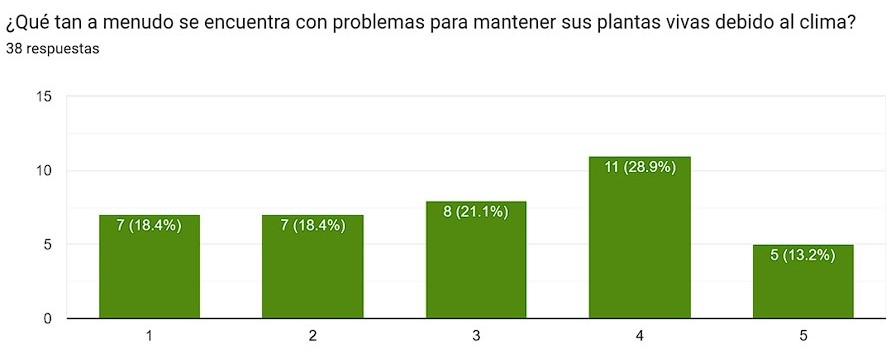
\includegraphics[width=.8\textwidth]{img/Empresa/encuesta1.jpg} 
    \caption{Problemas para mantener con vida sus plantas}
\label{fig:encuesta1}
\end{figure}

El porcentaje de personas que presentan problemas para mantener sus plantas vivas por el clima ver figura \ref{fig:encuesta1}.

\begin{figure}[H]
    \centering	
    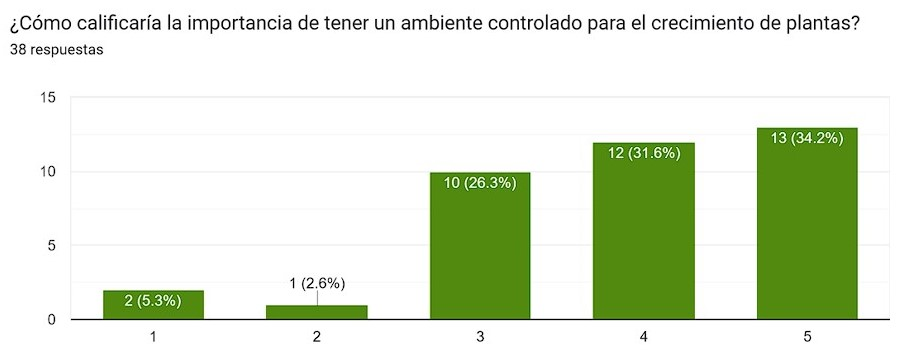
\includegraphics[width=.8\textwidth]{img/Empresa/encuesta2.jpg} 
    \caption{Importancia de ambiente controlado}
\label{fig:encuesta2}
\end{figure}

Percepción de la importancia de controlar el ambiente para el correcto crecimiento de plantas ver figura \ref{fig:encuesta2}.

\begin{figure}[H]
    \centering	
    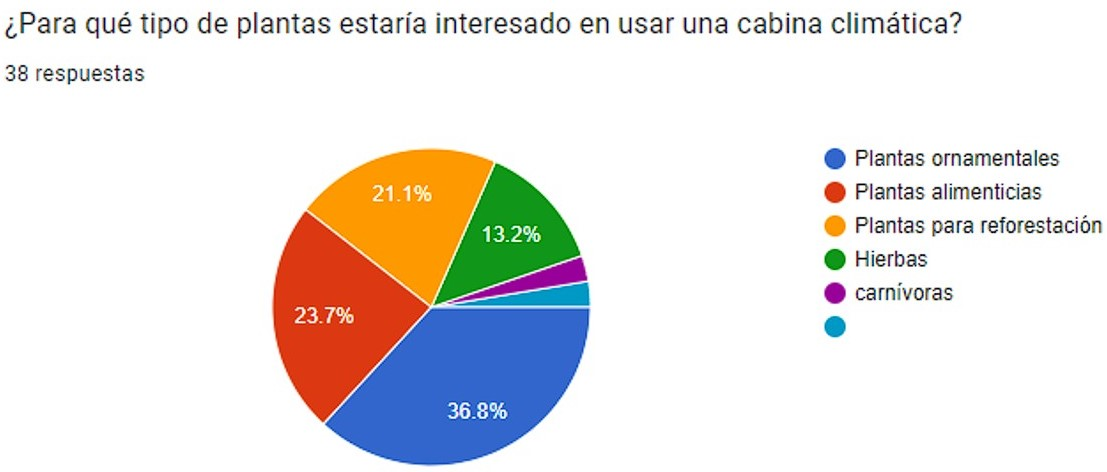
\includegraphics[width=.8\textwidth]{img/Empresa/encuesta3.jpg} 
    \caption{Importancia por tipos de planta}
\label{fig:encuesta3}
\end{figure}

Es importante recalcar que más del 40\% de los encuestados utilizarían el producto con fines de reforestación y producción de alimentos, incluso con mayor porcentaje de la población que la utilizaría en su casa u oficina ver figura \ref{fig:encuesta3}.

\begin{figure}[H]
    \centering	
    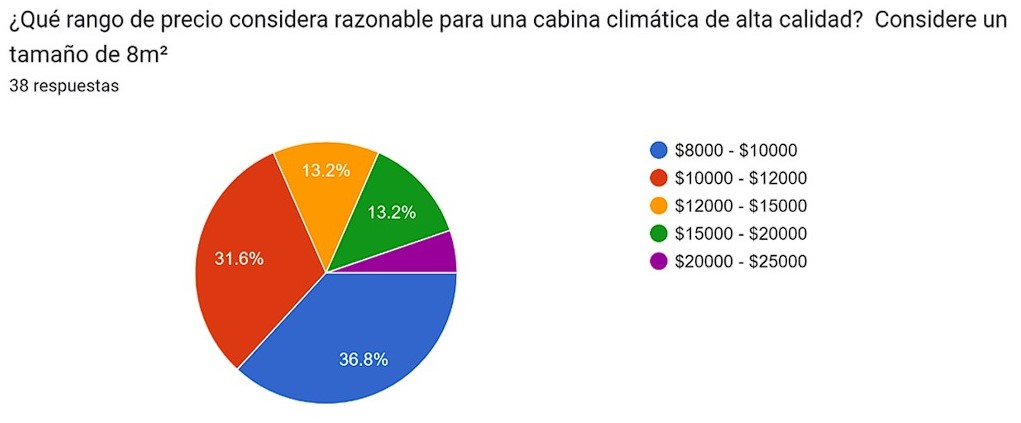
\includegraphics[width=.8\textwidth]{img/Empresa/encuesta4.jpg} 
    \caption{Rango de precios}
\label{fig:encuesta4}
\end{figure}

\section{Requisitos Municipales}
\label{sec:requisitosMunicipales}

\includepdf[pages=-]{chapters/RequisitosMunicipales.pdf}
